\chapter{Related Work}
\label{ch:related_work}
This chapter describes the current state of the stepper motor controllers in the Robotics group and the efforts to improve it.
Ongoing efforts to use program embedded systems in the Rust programming language is also described, both in the context of our research group and also in general.
Finally, similar projects - either software or hardware wise are reported.

\section{KM2}
\label{sec:km2}
In the Robotics and AI research group, currently a second generation of the KM2 stepper motor controller is widely in use.
A render of the KM2 controller can be seen in the figure~\ref{fig:km2render}.
It is used primarily by the students of the BPC-PRP course for driving a simple differentially driven robot.
The controller utilizes an ATMega8 paired with two stepper motor controllers DRV8825, that are utilized in the form of breakout boards generally used in the now obsolete RAMPS boards.
The motor controller is controlled using the I\textsuperscript{2}C bus.
There are two major shortcomings of the driver - the used controller's I\textsuperscript{2}C peripheral's clock-stretching is not compatible with Raspberry Pi's, causing problems on clock speeds higher than 30 kHz.
The second shortcoming are the used driver chips, that are quite loud and do not support contemporary advanced features.
The boards for 3D printers are also reportedly not well designed and they may \hl{overheat}~\cite{prusa_rambo}.

\begin{figure}[H]
    \centering
    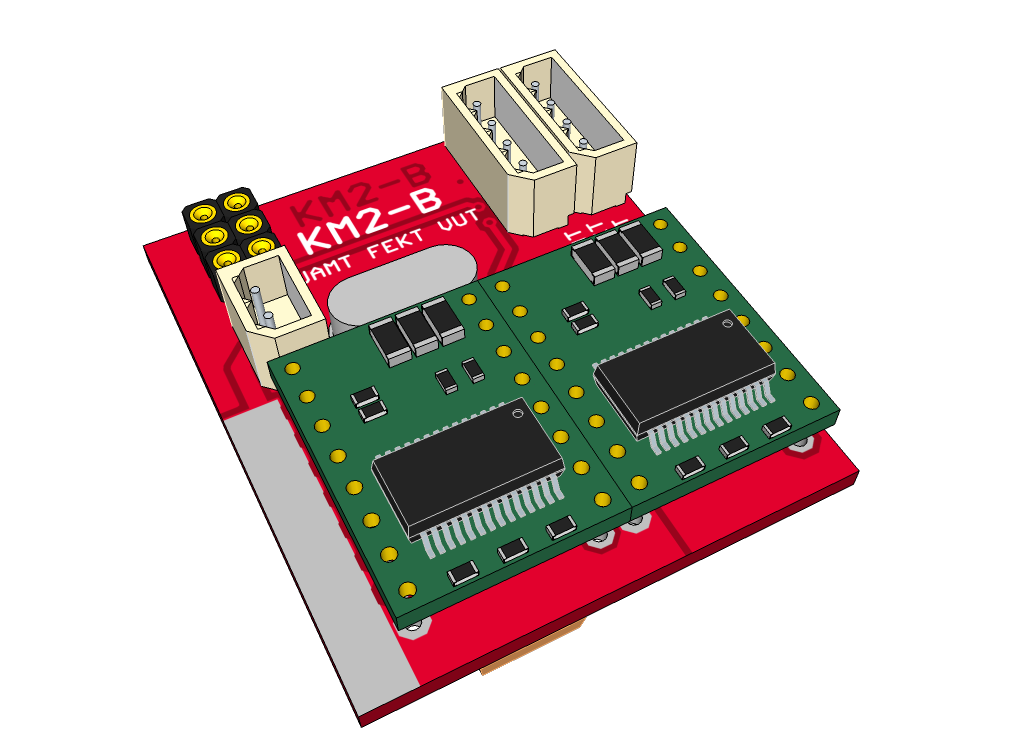
\includegraphics[width=0.5\textwidth]{obrazky/km2render}
    \caption{KM2 motor controller render~\cite{noauthor_km2renderpng_nodate}.}
    \label{fig:km2render}
\end{figure}

\section{KM3}
\label{sec:km3}
The KM3 (or KM2-C) was supposed to be a successor to the previously described KM2 controllers and it aimed to mainly solve the clock stretching problem by utilizing an STM32F031 MCU.
Another advantage of this revision was that the breakout boards for motor driver chips were replaced with driver chips soldered directly on the driver PCB (Printed Circuit Board).
The controller can be seen in the figure~\ref{fig:km3}.
Even though the new MCU was an improvement over the ATMega8, it proved to be the bottleneck for implementing new functionality to the motor controller as the MCU has very limited memory, both FLASH and RAM and peripherals.
For example, the lack of pins made it impossible to directly generate pulses to control the STEP/DIR interface of the motor drivers chip and the control had therefore be done manually in software.
Also the fact, that the MCU utilizes a Cortex-M0 core means that the support for atomic instructions mis missing, making it hard to work with guarantees about memory safety in cases of interrupt routine being called during memory manipulation

We developed the Rust firmware~\cite{noauthor_robotics-butkm3-rs_2020} for this board and concluded that the board and its design may be suitable for the students' robot projects, but it is way too limited to be used in more serious projects.
We also concluded that the hardware used is now overcome and the development of this board shall not be further pursued as the technology it's been designed upon as well as its goals have been considered obsolete.

\begin{figure}[H]
    \centering
    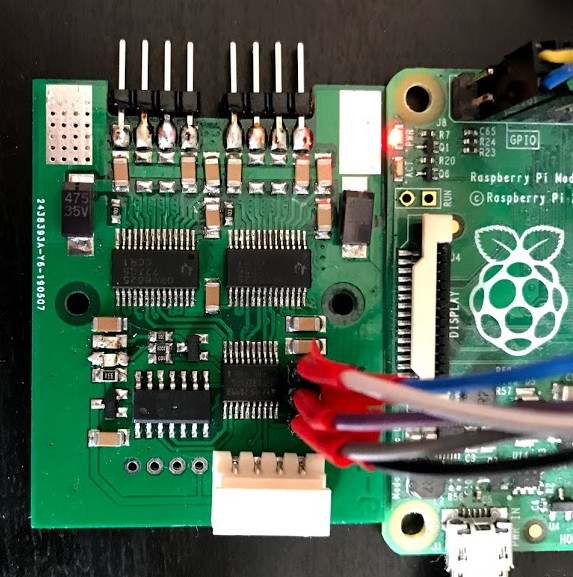
\includegraphics[width=0.7\textwidth]{obrazky/km3}
    \caption{The KM3 motor controller connected to a Raspberry Pi~\cite{noauthor_km2renderpng_nodate}.}
    \label{fig:km3}
\end{figure}

\section{DC Motor}
\label{sec:dcmotor}
The DC Motor is a custom-developed DC (Direct Current) motor controller developed in the Robotics \& AI research group.
It was designed to feedback control DC motors, primarily DC motors manufactured by Maxon and therefore provide a cheaper alternative to the Maxon EPOS motor controllers.
The driver alongside with a connected Maxon DC motor can be seen in the figure~\ref{fig:dcmotor}.
Originally, the firmware for the motors, developed by Frantisek Burian, Ph.D., implemented current control and velocity control.
However, the firmware exhibited unwanted behavior, such as extreme motor temperature rises and unwanted high-pich noise.
After consultation with Lukas Kopecny Ph.D., we decided to rewrite the firmware in Rust and get rid of the current controller, with the reasoning that current control of such low inductance motor makes not much sense and instead replaced it with some form of current limiting and failsafe overcurrent stops.
The new firmware alongside with some hardware modifications was successfully deployed to 7 DC Motor drivers as a part of the exhibition robots for the Technical Museum in Brno where they worked better than with the original firmware.

This driver was the first embedded project that used the Rust programming language for the development of the firmware.
We believe that using the language was the right choice and not only made the firmware simpler to use, but also made it possible to develop it in such short small time.
It can be said that the work on the firmware for this board laid the foundation for the work on this thesis.

\begin{figure}[H]
    \centering
    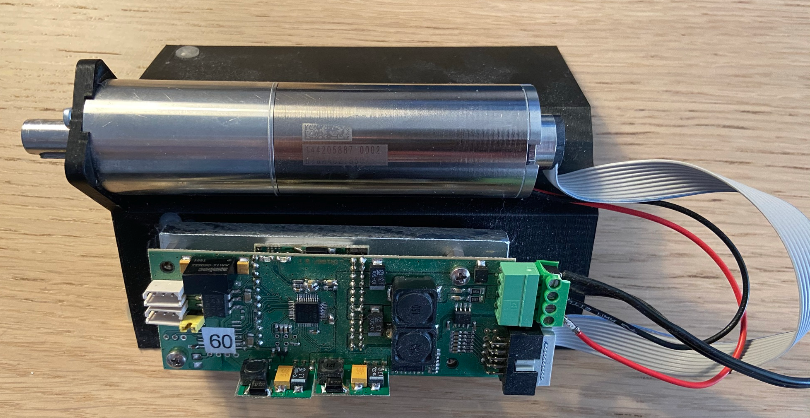
\includegraphics[width=0.7\textwidth]{obrazky/dcmotor}
    \caption{The DC Motor driver with a connected Maxon DC motor.}
    \label{fig:dcmotor}
\end{figure}

\section{Mechaduino}
\label{sec:mechaduino}
Mechaduino is a project that aims to create a servo motor out of a stepper motor.
The creators achieve that by mounting a PCB on the back of the motor that contains the power stage a MCU and a 14-bit magnetic encoder~\cite{noauthor_mechaduino_nodate}.
The mounting on the back of the stepper motor can be seen in the figure~\ref{fig:mechaduino}.
The big advantage that this project brings is integration of the whole system de-facto into the motor, removing any need for a controller board.
On the other hand, the controller doesn't leverage any existing stepper motor controller solution and instead implements the servo control manually.
When compared to our proposed solution, the Mechaduino has many advantages, even though it is only capable of controlling only one motor, it contains the encoder for feedback control and implements servo control algorithms out of the box.
On the other hand, our proposed solution leverages a state-of-the-art stepper motor controller ICs (Integrated Circuit), making it potentially less error prone and better for future use and development.
If there was a semestral thesis and preliminary market research preceeding this project, the Mechaduino would provide valuable information to improve the design of our project.

\begin{figure}[H]
    \centering
    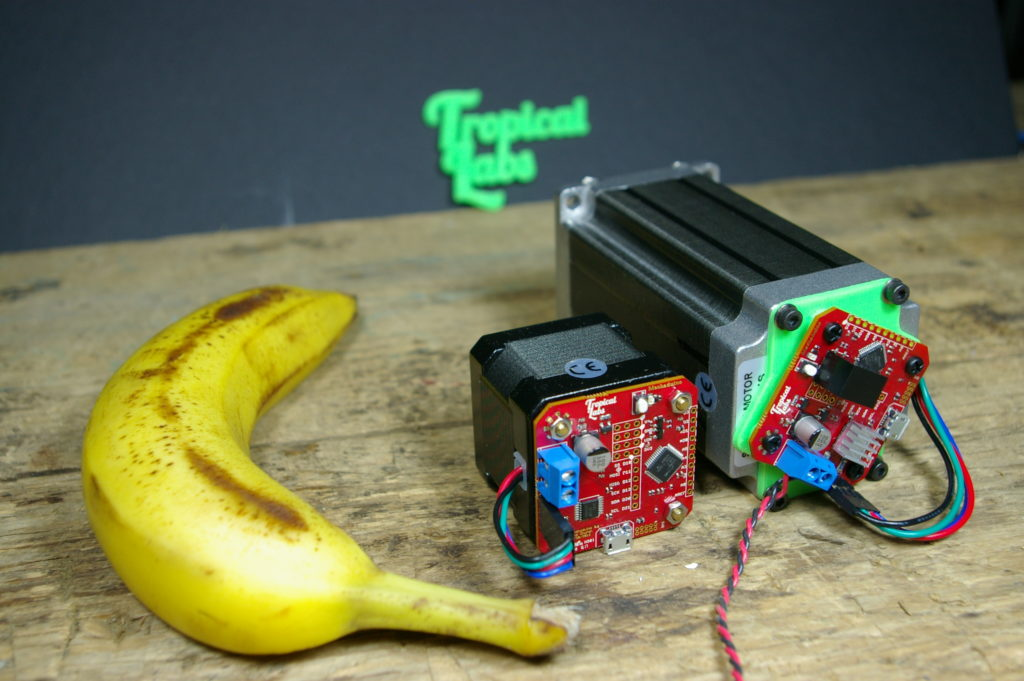
\includegraphics[width=0.7\textwidth]{obrazky/mechaduino}
    \caption{The Mechaduino controller boards mounted on the back of a stepper motors~\cite{noauthor_mechaduino_nodate}.}
    \label{fig:mechaduino}
\end{figure}

\section{Flott}
\label{sec:flott}
Flott is a set of libraries suitable for developing motion controllers in the Rust programming language\cite{noauthor_flott_nodate}.
It is a relatively new project, but as of now, it contains an abstraction layer for stepper motors and acceleration ramp generator.
The project is taking a different approach to controlling stepper motors as we are.
It aims to utilize software pulse generation instead of timers and uses variable step period in ramp generation.
Even though this is a valid approach we chose to not follow this model and instead implement this asynchronously using the MCU peripherals.
On the other hand the Flott project might be a great source of inspiration for future development and maybe sometimes the SM4 motor controller might utilize it.

\section{Takeaways from related work}
\label{sec:related-work-takeaways}
The past stepper motor development efforts in the Robotics \& AI research group showed the current solutions weak spots and advantages, which resulted in the following directions of the development of this project:
\begin{itemize}
    \item The project shall use a powerful, modern and capable MCU to be capable to fully support various features of the controller even in the future.
    \item The project shall use the state-of-art motor controller ICs.
\end{itemize}

The DC Motor project showed us, that writing a fully functional embedded firmware is not only a possible but a very viable option.

The Mechaduino project serves as a great inspiration into what can be achieved in servo motor based on a stepper motor.

Flott shows us that there are more people trying to achieve building a motion controllers in Rust and that we can get inspired from and share knowledge with.
We've been in contact with the Flott creator and consulted some ideas with them.
